\usetikzlibrary{arrows.meta}
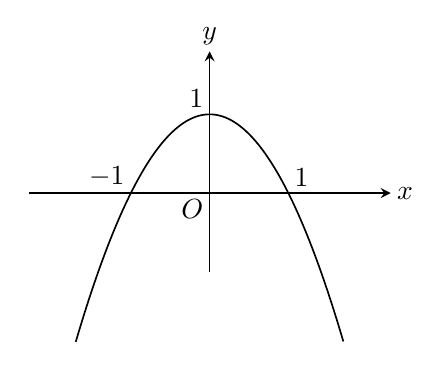
\begin{tikzpicture}[x=1cm,y=1cm,line width=.6pt,>=stealth]
\draw[->] (-2.3,0)--(2.3,0) node[right,inner sep=0pt,xshift=2pt] {$x$};
\draw[->] (0,-1)--(0,1.8) node[above,inner sep=0pt,yshift=2pt] {$y$};
\draw[domain=-1.7:1.7,samples=121] plot (\x,{1-\x*\x});
\node[above left,inner sep=0pt,xshift=-2pt,yshift=2pt] at (0,1) {$1$};
\node[above left,inner sep=0pt,xshift=-2pt,yshift=2pt] at (-1,0) {$-1$};
\node[above right,inner sep=0pt,xshift=2pt,yshift=2pt] at (1,0) {$1$};
\node[below left,inner sep=0pt,xshift=-2pt,yshift=-2pt] at (0,0) {$O$};
\end{tikzpicture}
